\section{Was ist Ethereum?}
\textit{Ethereum} ist eine open-source Blockchain und wird vor allem zum Erstellen von dezentralen Programmen bzw. Smart Contracts (\ref{l_smart_contracts}) verwendet.
Die Ethereum-Blockchain verwendet die Kryptowährung \textit{Ether (abgekürzt ETH, $\Xi$)} als Zahlungsmittel für Transaktionsverarbeitungen. Es können jedoch beliebige weitere Währungen -- sogenannte Tokens (\ref{l_tokens}) -- erzeugt werden, welche dann für Ether gehandelt werden können.

Ether ist zurzeit die Kryptowährung mit der zweitgrößten Marktkapitalisierung (Platz 1 \textit{Bitcoin}, Platz 3 \textit{Ripple}). \cite[Wikipedia, Ethereum]{Ethereum_Wikipedia}.
Im Gegensatz zu Bitcoin wird Ethereum nicht nur als Währung verwendet, sondern bietet auch eine Plattform für DApps (Decentralized Apps) (\ref{l_dapps}), die aus Smart Contracts bestehen.
 
Ethereum ist, als Blockchain, ein verteiltes System und ist ein Peer-to-Peer-Netzwerk bestehend aus \textit{Nodes}, also ohne zentrale Server (im Gegensatz zur Client-Server-Architektur).
Um am Netzwerk teilzunehmen, benötigt man einen Ethereum-Client, welcher sich mit dem Netzwerk synchronisiert, also Transakationen herunterlädt und überprüft.
Sogenannte \textit{Full Nodes} speichern die gesamte Blockchain und \textit{Light Nodes} nur einen Teil des Netzwerks; außerdem gibt es \textit{Mining Nodes} (\ref{l_mining}).
Die Ethereum-Blockchain ist derzeit 337 GB groß.

\section{Geschichte von Ethereum}
Das Whitepaper wurde 2013 veröffentlicht, 2014 folgte im \textit{Ethereum Yellow Paper} die formale Spezifikation und das Design der EVM (\ref{l_evm}). 2015 wurde das Netzwerk gestartet. Nach nur sieben Monaten -- am 29. Februar 2016 -- erreichte Ethereum eine Marktkapitalisierung von 500 Millionen US-Dollar. Nur zwei Wochen darauf hatte sich diese nochmals -- auf eine Milliarde US-Dollar -- verdoppelt.

\subsection{Ethereum Hard Fork, Ethereum Classic}\label{l_hard_fork}
\textit{The DAO} ist die bekannteste DAO (Decentralized Autonomous Organization)\footnote{eine Organisation, deren Managementstruktur und -regeln digital und unveränderbar durch einen Smart Contract festgeschrieben werden, diese dezentral ausgeführt werden und daher ohne konventionelle Entscheidungsgremien auskommt}, die bisher in der Ethereum-Blockchain implementiert wurde. Sie wurde von der Firma \textit{Slock.it} entwickelt und veröffentlicht. Grob zusammengefasst besteht die Aufgabe von The DAO darin, Ether durch Verkauf von Stimmberechtigungsanteilen einzunehmen, ein Entscheidungsgremium über die Verwendung des gesammelten Ethers abzuhalten und entsprechend das gesammelte Ether zu überweisen. Es handelt sich also um eine autonome und automatisierte Investmentfirma. The DAO wurde im April 2016 in die Blockchain hochgeladen und durchlief ein Crowdfunding bis zum 28. Mai 2016 (gekauft wurde mit der Kryptowährung Ether). The-DAO-Token, die zur Stimmabgabe für die in The DAO getroffenen Entscheidungen berechtigen, können auf diversen Kryptobörsen gehandelt werden.

Am 17. Juni 2016 hat ein Unbekannter durch einen Fehler im Smart Contract von The DAO 3.6 Millionen Ether unbrauchbar gemacht. Diese waren zum damaligen Zeitpunkt mehr als 65 Millionen Euro wert. Ein Hard Fork, der den Angriff rückgängig macht, war in der Community sehr umstritten, wurde dann aber in einer Abstimmung beschlossen. Durch diesen Hard Fork wurden der angreifenden DAO die Ethers entzogen; daraus entstanden zwei Blockchains, von denen die ursprüngliche als \textit{Ethereum Classic (ETC)} weitergeführt wird. Die \textit{Ethereum Foundation} hat anhand verschiedener Metriken und der Abstimmung der Community entschieden, ihre Entwicklungstätigkeit nur auf die abgespaltene Hauptblockchain (weiterhin \textit{Ethereum} genannt) zu beschränken und sich nicht mit Ethereum Classic zu beschäftigen.

Ethereum Classic wurde Anfang 2019 zum Ziel von Hackern, die das Netzwerk angriffen und Kryptowährung im Gegenwert von etwa 1.5 Millionen US-Dollar erbeuteten. Sie hatten sich dazu offenbar Kontrolle über das Mining-Netzwerk verschafft und die Blockchain reorganisiert, sodass die Einheiten der Währung doppelt ausgegeben werden konnten. Der Handelsplatz \textit{Coinbase} stoppte daraufhin den Handel mit ETC.

\subsection{Kursentwicklung}
\begin{figure}[H]
    \centering
    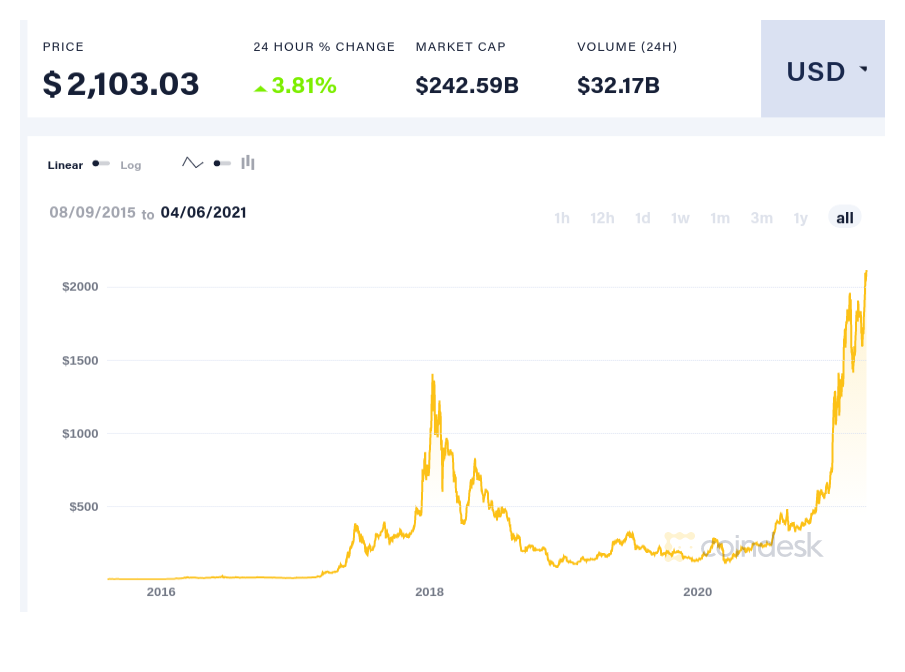
\includegraphics[width=0.7\linewidth]{images/eth-kurs.png}
    \caption{ETH-Kurs in US-Dollar}
\end{figure}

Im Januar 2018 stieg der Ethereum-Kurs sehr stark, sank danach jedoch wieder ab. Derzeit ist er wieder am Steigen.

\section{Ethereum Virtual Machine (EVM)}\label{l_evm}
Die EVM ist komplett isoliert -- Code, der in ihr läuft, hat also auch keinen Zugriff auf das Dateisystem, Netzwerk, andere Prozesse etc.

\subsection{Contracts}
Es gibt External Accounts (Public-Private-Schlüsselpaare) welche vor allem Endnutzer darstellen und Contract Accounts, welche per Smart Contract-Code gesteuert werden. Beide Account-Arten haben eine Balance in Ether, welche durch Transaktionen verändert werden kann.

\subsection{Transaktionen}
Eine Transaktion ist eine Nachricht von einem Account zu einem anderen und kann Binärdaten (eine \textit{Payload}) und Ether beinhalten. Sollte der Target Account Code beinhalten, so wird dieser ausgeführt und diesem wird die Payload als Input-Daten zur Verfügung gestellt.

Sollte eine Transaktion keinen Target Account gesetzt haben bzw. ist dieser auf \texttt{null} gesetzt, so wird mithilfe der Transaktion ein neuer Contract erstellt. Die Payload dieser Transaktion wird dann ausgeführt und der Output der Transaktion als Code des Contracts gespeichert. (Also es wird eigentlich nicht der Contract Code als Payload geschickt, sondern Code, welcher, wenn ausgeführt, den Contract Code zurückliefert.)

\subsection{Gas}
\textit{Gas} muss gezahlt werden, um eine Transaktion durchzuführen oder einen Contract auszuführen. Der genaue Preis wird durch Angebot/Nachfrage bestimmt: Die Miner werden eine Transaktion nicht durchführen wollen, wenn die Entschädigung zu gering ist.

Siehe \url{https://ethereum.org/en/eth2}.

\section{Konsens-Mechanismen}
\begin{quote}
\begin{itshape}
"One major obstacle to overcome is what (in Bitcoin terms) is called a "double-spend attack": What happens if two transactions exist in the network that both want to empty an account? Only one of the transactions can be valid, typically the one that is accepted first. The problem is that “first” is not an objective term in a peer-to-peer network.

The abstract answer to this is that you do not have to care. A globally accepted order of the transactions will be selected for you, solving the conflict. The transactions will be bundled into what is called a “block” and then they will be executed and distributed among all participating nodes. If two transactions contradict each other, the one that ends up being second will be rejected and not become part of the block.

These blocks form a linear sequence in time and that is where the word “blockchain” derives from. Blocks are added to the chain in rather regular intervals -- for Ethereum this is roughly every 17 seconds.

As part of the “order selection mechanism” (which is called “mining”) it may happen that blocks are reverted from time to time, but only at the “tip” of the chain. The more blocks are added on top of a particular block, the less likely this block will be reverted. So it might be that your transactions are reverted and even removed from the blockchain, but the longer you wait, the less likely it will be."
\end{itshape}
\ \cite[Solidity Docs, Blocks]{Blocks_Solidity}
\end{quote}

Aktuell verwendet Ethereum einen Proof-of-Work-Mechanismus, dieser soll jedoch im Laufe der Entwicklung durch einen Proof-of-Stake-Mechanismus ersetzt werden.

\subsection{Proof-of-Work (PoW)} \label{l_mining}
Ein \textit{Block} auf der Blockchain besteht aus mehreren Transaktionen; diese Transkationen werden durch \textit{Mining} (auf der CPU\footnote{Central Processing Unit}/GPU\footnote{Graphics Processing Unit}/ASIC\footnote{Application-Specific Intregrated Circuit}) verifiziert.

Das Problem mit PoW ist, dass es \textbf{sehr viel Energie verbraucht}, da ein großer Rechenaufwand besteht.

\subsection{Proof-of-Stake (PoS)}
Bei PoS setzen mehrere Nodes ihre eigenen Kryptowährungen für die Transaktionsvalidierung ein; diese werden "Staker" genannt. Je größer der Betrag des Einsatzes und je länger die Dauer des Einsatzes, desto besser sind die Chancen des Stakers, die Verantwortung für die Transaktionsvalidierung zu erhalten.

Alle Kryptowährungen in diesem Netzwerk sind bereits erstellt, und es gibt kein Mining. Damit entfällt der Rechenaufwand. Auch die ständige Aufrüstung der Hardware und die steigenden Energiekosten entfallen. Der Prozess der Transaktionsvalidierung wird "Forging" genannt. Außerdem muss nicht das ganze Netzwerk am Validierungsprozess beteiligt sein.

% TODO: besser erklären, dass währung beiseite gelegt wird

\cite[vgl. Medium, PoW vs PoS]{PoW_vs_PoS}


\section{Smart Contracts}\label{l_smart_contracts}
Smart Contracts sind Programme, die automatisch ausgeführt werden, sobald eine in dem Contract festgelegte Summe in Ether überwiesen wurde. Damit ist keine (manuelle) Überprüfung eines Zahlungseingangs mehr erforderlich, denn die Überweisung startet direkt die im Programm festgelegte Gegenleistung.
Jede Transaktion wird innerhalb der gesamten Blockchain -- also auf allen mit dem Netzwerk verbundenen Geräten -- gespeichert. Das dezentrale Konzept der Blockchain prüft die Integrität der gesamten Datenbank permanent.

Smart Contracts werden meist in der für Ethereum eigens entwickelten Programmiersprache \textit{Solidity} geschrieben (weitere Sprachen sind z. B. \textit{Serpent, Yul, LLL, Mutan}). Sie werden dann in Bytecode übersetzt und auf der \textit{Ethereum Virtual Machine (EVM)} ausgeführt.

Ein Problem von Smart Contracts ist, dass Bugs von allen ersichtlich sind, da der Source Code von allen eingesehen werden kann, diese Fehler allerdings kaum behebbar sind (siehe das \textit{The DAO}-Problem (\ref{l_hard_fork}).

Smart Contracts können zum Beispiel Transaktionen abbilden oder Service-Level-Agreements umsetzen. \textbf{Smart Contracts an sich sind keine rechtlichen Verträge}, aber natürlich kann im Vertrag beschlossen werden, dass ein gewisser Smart Contract Teil vom Vertrag und bindend ist.

\cite[vgl. Wikipedia, Ethereum]{Ethereum_Wikipedia}


\section{Anwendungen}
\subsection{Decentralized finance (DeFi)}
\begin{quote}
\begin{itshape}
"Dezentralisierte Finanzmärkte (englisch decentralized finance -- DeFi) sind experimentelle neuartige Formen von Finanzmärkten, welche auf Smart Contracts und dezentralisierten autonomen Organisationen auf Blockchains basieren. Im Gegensatz dazu basieren traditionelle Finanzmärkte auf zentralen Finanzintermediären, wie zum Beispiel Börsenmakler, Wertpapierhändlern und Banken. Diese zentralen Intermediäre werden durch zentralisierte Informationssysteme unterstützt. Intermediäre existieren in einem dezentralen Finanzmarkt, jedoch sind diese durch Smart Contracts realisiert und nicht durch eine oder wenige Organisationen."
\end{itshape}
\ \cite[Wikipedia, Dezentralisierte Finanzmärkte]{Dezentralisierte_Finanzmaerkte}
\end{quote}

Folgende Vorteile ergeben sich daraus:
\begin{itemize}
\item Volle Transparenz für die Teilnehmer einer Blockchain. Auf einer öffentlichen Blockchain kann theoretisch jeder diese einsehen
\item Beliebige komplexe dezentrale Finanzmärkte lassen sich abbilden
\item Geringere Transaktionskosten -- insbesondere zwischen verschiedenen Wirtschaftsräumen, aber auch innerhalb eines Wirtschaftsraumes
\item Smart Contracts können von jedem eingesehen und getestet werden
\item Blockchains garantieren basierend auf den Informationen innerhalb der Blockchain korrekte Vertragsausführung
\item Anonymität oder Pseudonymität
\end{itemize}

Und folgende Nachteile:
\begin{itemize}
\item Smart Contracts werden in Software abgebildet und derzeit gibt es noch wenig Wissen wie man komplexe dezentralisierte Finanzmärkte testen kann
\item Es ist schwierig sein Recht durchzusetzen, da Smart Contracts -- sofern es nicht im Smart Contract vorgesehen ist -- nicht rückgängig machbar sind. Das Rechtswesen hat bisher wenig Urteile zu dieser Form der Organisation gefällt und es gibt nur rudimentäre Gesetze. Dezentrale Finanzmärkte sind nochmal komplexer als "normale" Verträge und somit ist es rechtlich noch komplizierter
\item Es gibt noch kaum Erfahrung auf dem Gebiet der Aufsicht und Analyse von Blockchains
\item Blockchain-externe Informationsquellen können kein Vertragsgegenstand sein, da sie nicht eindeutig nachvollziehbar sind
\end{itemize}


\subsection{Decentralized Apps (DApps)}\label{l_dapps}
DApps sind Programme, die auf einer Blockchain und damit auf allen Nodes parallel ausgeführt werden. Am einfachsten stellt man sich eine DApp als eine Website vor. Während jedoch klassische Websites via API mit einem zentralen Server und ggf. Datenbanken verbunden sind, ist die DApp via Smart Contract mit der Blockchain verbunden. Die DApp "kauft" über den Smart Contract mittels Ether das \textit{Gas} -- anschaulich ein Treibstoff -- welches für ihre Ausführung auf der Blockchain benötigt wird.

Dies ist teurer und langsamer als das traditionelle Client-Server-Modell, bietet aber einige Vorteile: Auf zentralisierten Servern können Angreifer Daten manipulieren. Das dezentrale Konzept der Blockchain prüft jedoch die Integrität der gesamten Datenbank permanent. Somit sind dezentrale Apps fehlertolerant, unabänderlich und erleiden keine Verbindungsunterbrechungen.

\cite[vgl. Wikipedia, Smart Contracts]{Smart_Contract_Wikipedia}

\subsection{Collectibles, Spiele}
Siehe z. B. \cite[CryptoKitties]{CryptoKitties}, \cite[0xUniverse]{0xUniverse}

\section{Zukunft von Ethereum -- Ethereum 2.0}
Die größte Änderung ist die Umstellung von Proof-of-Work zu Proof-of-Stake.

\section{Anderes, häufig verwendete Begriffe}

\subsection{Wallet}
Eine Wallet speichert den Public und Private Key eines Accounts. Der Public Key ist zudem die Adresse des Accounts. Die Währung liegt nicht in der Wallet, sondern auf der Blockchain.

\subsection{Unterschied Token -- Kryptowährung?}\label{l_tokens}
Ein \textit{Kryptowährung} ist die native Währung einer Blockchain und diese wird vom Netzwerk ausgestellt bzw. man bezahlt sie, um Transaktionen zu tätigen. \textit{Tokens} hingegen bauen auf einer Blockchain auf.

Beispielsweise ist Ether die Kryptowährung von Ethereum, aber es gibt noch weitere Tokens, die auf der Plattform aufbauen (z. B. \textit{DAI}, \textit{LINK}).

Es gibt verschiedene \textit{Token Standards}, nach welchen ein Token erstellt wird. Aufbauend auf Ethereum gibt es beispielsweise \textit{ERC-20} (wird hauptsächlich als Währung verwendet) und \textit{ERC-721} (wird hauptsächlich für Collectibles verwendet).

Tokens besitzen nicht nur einen bestimmen Wert und können ausgetauscht werden, sondern können auch so designed sein, dass sie z. B. physische Vermögenswerte oder einen bestimmten Nutzen oder Service repräsentieren. Es gibt beispielsweise Krypto-Token, die materielle Vermögenswerte wie Immobilien und Kunst sowie immaterielle Vermögenswerte wie Rechenleistung oder Datenspeicherplatz repräsentieren.

\cite[vgl. Gemini, Cryptocurrencies vs Tokens]{Cryptocurrencies_vs_Tokens}

\subsection{Fiat Money}
Fiatgeld ist "klassisches" Geld, das vom Staat/einer Organisation verwaltet wird, wie Euro, US-Dollar etc.

\subsection{Stablecoins}
\textit{Stablecoins} sind Kryptowährungen, deren Preis möglichst stabil ist. Dies kann z. B. geschehen, indem der Preis an den aktuellen Wert einer Fiat-Währung gebunden wird.

Ein Beispiel wäre Tether (\textit{USDT}), wessen Wert an den US-Dollar gebunden ist. 1 USDT entspricht also \$1.00.

\subsection{Altcoins}
Als \textit{Altcoins} werden alle Kryptowährungen, Tokens und andere Assets bezeichnet, die nicht Bitcoin sind.